\section{Shared-reader results: the original primary analysis}
\label{sec:results}
Both frozen blocks completed, with all 768 planned logical attempts retained. The primary block issued 494 actual reader requests and reused 82 identical requests; the sensitivity block issued 182 and reused 10. No execution failure, output truncation, missing usage or schema-invalid response was recorded. Schema validity is partly enforced by the common grammar and is not evidence of recommendation correctness. Both provenance audits verified the saved inputs and requests.

\subsection{The primary contrast is positive but uncertain}
At 1,024 input tokens, catalog coverage produces 53/96 correct supported decisions (55.2\%), compared with 40/96 (41.7\%) for prompt hybrid. The paired world difference is 13.5 percentage points, with a 95\% stratified bootstrap interval of [0.0, 28.1]. Because this interval includes zero, the primary comparison does not establish clear superiority. The observed paired-world SD is 0.284, above the 0.20 planning floor. The achieved interval must therefore be read as observed, rather than as a guaranteed planning precision.

\begin{table}[htbp]
\centering\small
\begin{tabular}{lrrrrr}
\toprule
Method & Decision & Positive & Neg. rec. & Tokens & Gen. sec. \\
\midrule
Generic hybrid & 50.0\% & 4.2\% & 4.2\% & 1015 & 37.5 \\
Prompt hybrid & 41.7\% & 0.0\% & 16.7\% & 1013 & 36.6 \\
Facet hybrid & 35.4\% & 0.0\% & 29.2\% & 1012 & 35.6 \\
Catalog coverage & 55.2\% & 43.8\% & 33.3\% & 1016 & 34.0 \\
Full context & 56.2\% & 52.1\% & 39.6\% & 2099 & 67.1 \\
History ablation & 31.2\% & 35.4\% & 72.9\% & 1016 & 33.5 \\
\bottomrule
\end{tabular}

\caption{Primary results. Decision is correct supported decisions over all 96 queries; Positive is supported recommendations over 48 answerable queries; Neg.\ rec. is inappropriate recommendations over 48 negative queries. Tokens are mean input tokens per planned query; Gen.\ sec. is median generation-request elapsed time, charging the origin call for reused requests. Full context has its separate larger allowance.}
\label{tab:primary}
\end{table}

The difference is not a uniform improvement in caution and coverage. Catalog coverage answers 21/48 positive cases correctly, compared with none for prompt hybrid, but makes 16/48 inappropriate negative recommendations versus 8/48. Across paired queries, catalog coverage alone is correct on 26, prompt hybrid alone on 13, both on 27, and neither on 30. Always withholding scores 48/96 on this balanced task. Generic hybrid also scores 48/96, through two supported positive recommendations and 46 correct negative decisions. Neither aggregate accuracy nor a conservative response pattern alone demonstrates useful coverage.

\begin{figure}[htbp]
\centering
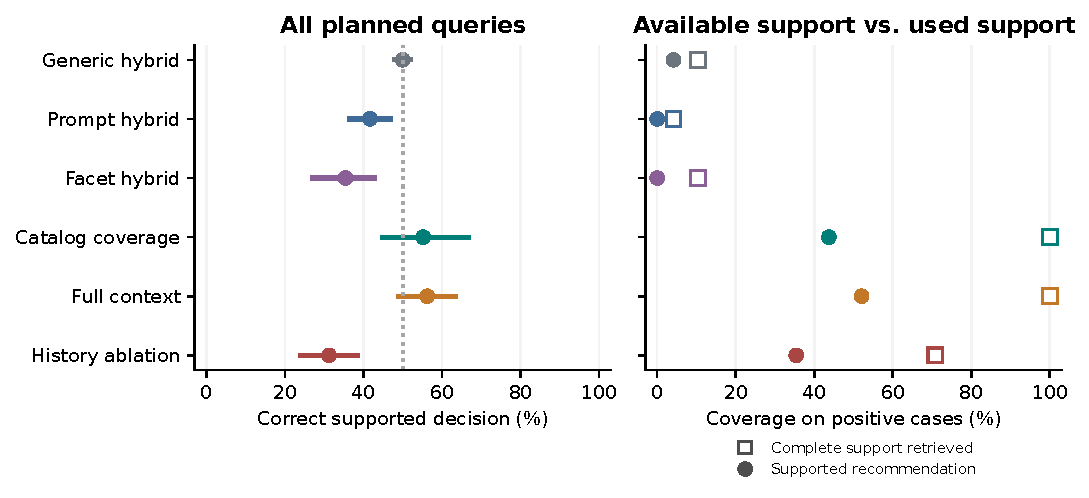
\includegraphics[width=\linewidth]{figures/primary/quality.pdf}
\caption{Primary decision quality and positive-case support. Left: method accuracy with world-bootstrap intervals; the dotted line is always withholding. Right: complete support retrieved versus correctly supported recommendations. Available evidence is necessary under this scorer but is plainly insufficient for this reader. Intervals describe resampling of the fictional worlds.}
\label{fig:quality}
\end{figure}

\subsection{Evidence selection and evidence use fail separately}
Catalog coverage and full context each supply a complete witness for all 48 positive cases. Prompt hybrid supplies one in only 2/48, and generic and facet hybrid in 5/48 each. The smaller input allowance can nevertheless hold a complete witness for every positive query, as the pre-results capacity audit establishes. These are selection failures under the implemented ranking and distractor distribution, not a proof that generic memory cannot represent the necessary facts.

Complete support does not solve utilization. Among catalog coverage's 48 positive cases, 21 succeed, 13 withhold despite complete support, 13 choose an inapplicable template, and one has invalid support bindings. Full context succeeds on 25, with six inappropriate withholds, 15 inapplicable choices and two binding failures. These descriptive categories do not isolate a causal effect of evidence availability from positions, aliases or other input changes. All supported positive decisions complete the mock workflow; this dependent consistency check adds no independent evidence of strategic usefulness.

Condition-level results expose a sharp boundary. At the primary cap, catalog coverage fails all 12 changed-objective queries despite retrieving their complete qualification support, while full context solves eight. In the first lexicographic withholding example, query \texttt{q0b2e9ee8ab}, primary attempt 167 correctly fills all four common qualification bindings but requests partner-specific facts that the qualification template does not require. Full-context attempt 211 selects the valid qualification template. This is a recorded alternative-scoping failure, not an explanation inferred solely from a score. Additional examples and all disagreements remain in the evidence package.

\subsection{Controls reveal costs of instructions and unresolved history}
Table~\ref{tab:contrasts} reports every frozen primary-block contrast. Catalog coverage exceeds facet hybrid descriptively, so generic diversity does not close the observed gap in this configuration. The prompt-specialized control scores below the generic control. This combines instruction effects with evidence displaced by the longer checklist under a total-token cap; it does not isolate the effect of wording alone.

\begin{table}[htbp]
\centering\small
\begin{tabular}{lrr}
\toprule
Paired contrast & Difference (pp) & 95\% interval (pp) \\
\midrule
Catalog coverage $-$ prompt hybrid & 13.5 & [0.0, 28.1] \\
Catalog coverage $-$ facet hybrid & 19.8 & [4.2, 38.5] \\
Prompt hybrid $-$ generic hybrid & $-8.3$ & [$-15.6$, $-1.0$] \\
Catalog coverage $-$ history ablation & 24.0 & [17.7, 31.3] \\
Full context $-$ catalog coverage & 1.0 & [$-11.5$, 13.5] \\
\bottomrule
\end{tabular}
\caption{World-paired effects at the primary cap. Only the first contrast is primary; the others explain behavior without a multiplicity-adjusted superiority claim. Full context is separately costed. An interval spanning zero does not establish equivalence.}
\label{tab:contrasts}
\end{table}

Removing supersession resolution lowers catalog coverage from 53/96 to 30/96 decisions. The current-view method is correct alone on 23 paired queries; the history ablation is never correct alone. The ablation cites obsolete or ineligible evidence on 32 attempts and recommends on 35/48 negative cases. Its positive support availability also falls to 34/48, so this comparison includes stale-evidence crowding as well as interpretation of replacement links. It supports resolving the explicit replacement semantics used here, not a claim of general learned belief revision.

Transition behavior remains incomplete. Catalog coverage is correct both initially and after weak feedback in 6/12 worlds (6/8 conditional on initial correctness). It is correct both before and after the approved policy revision in only 1/12 (1/6 conditional on the earlier decision). After account requalification and the later evidence correction, it is correct on both in 7/12 (7/7 conditional); the history ablation achieves 0/12. These paired snapshots do not test an agent updating a running action or learning from its own experience.

\subsection{Larger inputs help without establishing reliability}
At 1,536 input tokens, catalog coverage scores 59/96 (61.5\%) and prompt hybrid 42/96 (43.8\%). The exploratory paired difference is 17.7 points [10.4, 26.0]. It does not replace the uncertain primary result. Positive support availability rises to 36/48 for prompt hybrid and stays at 48/48 for catalog coverage; supported positive recommendations are 13/48 and 30/48 respectively. Both methods recommend inappropriately on 19/48 negative cases.

Catalog coverage now solves 10/12 changed-objective queries, versus zero at the smaller allowance. Extra context changes more than the existence of a sufficient witness: its contents, positions and source labels also change. This improvement therefore cannot be attributed to missing prerequisites alone. Conversely, prompt hybrid gains 13 supported positive recommendations but loses 11 correct negative decisions relative to its primary-block result. More evidence is not a monotonic safety improvement.

\subsection{Computation and the exact-rule reference}
Mean primary input usage is 1,015.6 tokens for catalog coverage, 1,013.0 for prompt hybrid and 2,098.6 for full context. Their median generation times are 34.0, 36.6 and 67.1 seconds. Estimated component totals, charging each method its associated embedding origins and logical generation work, are 3,389.9, 3,605.8 and 6,557.5 seconds respectively. These shared-run estimates support a descriptive resource comparison, not a measured commercial lifecycle-cost advantage or a proof that the methods are equally accurate.

Across both blocks, 676 physical requests consume 882,141 input and 119,434 output tokens. Unique associated embedding work comprises 313 event and 24 query representations, taking 41.8 seconds in total. That work is already nested in observed retrieval time. The blocks consume 30,853.6 seconds (8.57 hours) of elapsed server time; local API charges are zero, while hardware value, energy, extraction and curation costs are unknown. Full computation receipts distinguish actual shared work from per-method charges.

The exact SQLite reference solves all 96 queries with zero generation calls and 0.084 seconds of recorded policy-evaluation time, excluding loading and other setup. That timing is not comparable to an end-to-end model deployment. Its correctness is nevertheless a substantive boundary: when the facts and eligibility language are already explicit, formal rule evaluation is sufficient. The learned-reader results must not be used to argue that an LLM is necessary for this contract.
